\documentclass[prd,amsmath,amssymb,floatfix,superscriptaddress,nofootinbib]{revtex4-1}
\usepackage{bm}
\usepackage{amsmath}
\usepackage{epsfig}
\usepackage{color}
\usepackage{natbib}
\usepackage{textcase}
\usepackage{graphicx}
\usepackage{ifthen}
\usepackage{xstring}
\usepackage{graphicx}
\usepackage[utf8]{inputenc} 
\usepackage{amssymb}
\usepackage{latexsym}
\usepackage{epstopdf}
\epstopdfsetup{update}
\DeclareGraphicsExtensions{.ps, .png}
\epstopdfDeclareGraphicsRule{.ps}{pdf}{.pdf}{ps2pdf -dEPSCrop -dNOSAFER #1 \OutputFile} 
\usepackage{dcolumn} 
\usepackage{multirow}
\usepackage{appendix}
\usepackage{footnote}
\usepackage{tabularx,ragged2e,booktabs}
\usepackage[normalem]{ulem}
\usepackage{float}
\restylefloat{table}

\newcommand{\tauhi}{$\tau_{\rm hi}\,$}
\newcommand{\taulo}{$\tau_{\rm lo}\,$}

\newcommand{\refsec}[1]{section~\ref{sec:#1}}
\newcommand{\refeq}[1]{Eq.~(\ref{eq:#1})}
\newcommand{\refssec}[1]{section~\ref{subsec:#1}}
\newcommand{\reffig}[1]{Fig.~\ref{fig:#1}}
\newcommand{\refFig}[1]{Fig.~\ref{fig:#1}}
\newcommand{\curv}{{\cal R}}
\newcommand{\xef}{x_e^{\rm fid}}
\newcommand{\xmax}{x_e^{\rm max}}
\newcommand{\zmax}{z_{\rm max}}
\newcommand{\zmin}{z_{\rm min}}
\newcommand{\xemin}{x_e^{\rm min}}

\newcommand{\ra}{\rightarrow}
\def\max{_{\mathrm{max}}}
\def\lsim{\mathrel{\raise.3ex\hbox{$$<$$\kern-.75em\lower1ex\hbox{$\sim$}}}}
\def\gsim{\mathrel{\raise.3ex\hbox{$$>$$\kern-.75em\lower1ex\hbox{$\sim$}}}}

\newcommand{\beq}{\begin{equation}}
\newcommand{\eeq}{\end{equation}}

\newcommand{\bea}{\begin{eqnarray}}
\newcommand{\eea}{\end{eqnarray}}

\newcommand{\wh}[1]{\textcolor{blue}{#1}}
\newcommand{\ch}[1]{\textcolor{red}{#1}}

\def\mnras{Mon.\ Not.\ R.\ Astron.\ Soc.\ }
\definecolor{darkgreen}{cmyk}{0.85,0.2,1.00,0.2} 
\definecolor{purple}{cmyk}{0.5,1.0,0,0} 
\def\physrep{Phys.~Rep.}

\definecolor{ultramarine}{rgb}{0.07, 0.04, 0.56}
\definecolor{cadmiumgreen}{rgb}{0.0, 0.42, 0.24}
\definecolor{indigo(dye)}{rgb}{0.0, 0.25, 0.42}
\usepackage[linktocpage=true]{hyperref}
\hypersetup{
colorlinks=true,
citecolor=ultramarine,
linkcolor=cadmiumgreen,
urlcolor=indigo(dye),
pdfauthor={},
pdftitle={},
pdfsubject={}
}


\begin{document}
	
\title{Reionization Planck 2018 Notes}

\author{Chen Heinrich}
\author{Wayne Hu}
 
\maketitle

\section{Introduction}
\label{sec:intro}

Trying to collect all of our tests here.\\

List of tests:\\
\begin{itemize}
    \item {Direct MCMC chains
        \begin{enumerate}
            \item {PC zmax = 30}
            \item {PC zmax = 50}
            \item{Tanh model}
            \item{Two-parameter model with \taulo and \tauhi}
        \end{enumerate}
    }
    \item{Best-fit tests
        \begin{enumerate}
            \item {From the chains for the 2-parameter model, we found that if we restrict \tauhi $> 0.02$, we get that the ML model is: 
            \begin{itemize}
                \item {\tauhi = 0.0206}
                \item {\taulo = 0.0414} 
                \item {$z_{\rm re}$ = 6.29} 
                \item {$x_{e, \mathrm{hi}}$ = 0.0748}
                \item {-loglike = 499.5458} 
            \end{itemize}
            There is a difference of $\Delta \chi^2 = 2.6$, compared against the ML model from the full chain:
            \begin{itemize}
                \item {\tauhi = 0.00542}
                \item {\taulo = 0.0543} 
                \item {$z_{\rm re}$ = 7.68} 
                \item {$x_{e, \mathrm{hi}}$ = 0.0214}
                \item {-loglike = 498.2425} 
            \end{itemize}
             }
            \item{Using above information, we ran a best-fit search fixing \tauhi = 0.02 to find the best-fit model:
            \begin{itemize}
                \item {\tauhi = 0.02 (fixed)}
                \item {\taulo = 0.045 (c.f. 0.0414 from chains)} 
                \item {$z_{\rm re}$ = 6.67} 
                \item {$x_{e, \mathrm{hi}}$ = 0.073}
                \item {-loglike = 499.2914} 
            \end{itemize} 
            giving a difference of $\Delta \chi^2 = 2.1$  (c.f. 2.6 above).}\\
            Note: I need to update the plots with xe(z) to this model.
            \item{We also ran a chain fixing \taulo = 0.04, but I forgot what this was for ...}
        \end{enumerate}
        }
        
    \item {KDE tests
        \begin{enumerate}
            \item {The tanh model: direct MCMC, vs python (f = 0.10, 0.12, 0.14) and fortran version (0.14) - coming up}
            \item {The 2-parameter model: direct MCMC vs fortran version (f = 0.10, 0.12, 0.14) - coming up}
        \end{enumerate}
    }
    
\end{itemize} 



\begin{figure}
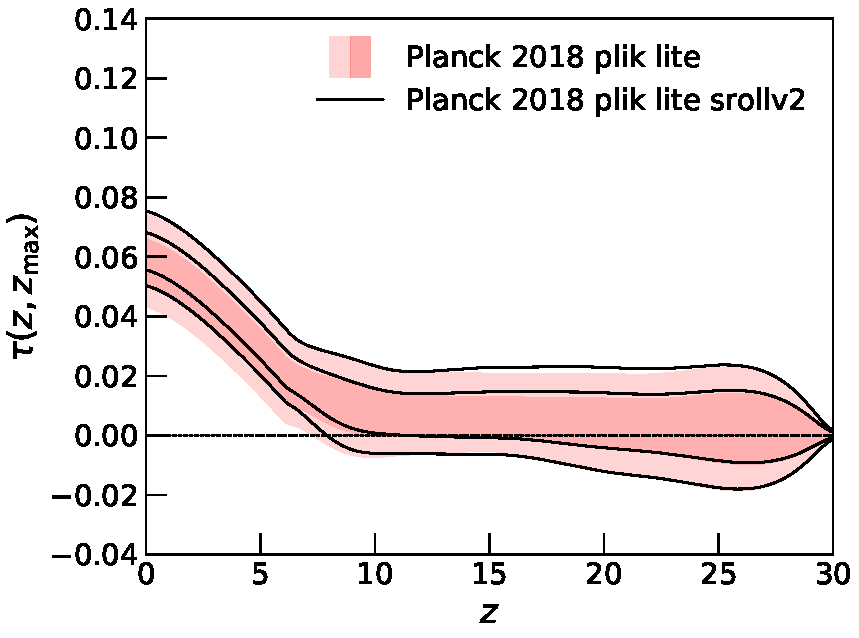
\includegraphics[width=0.65\textwidth]{results/direct_mcmc/pl18_plots_zmax30/plot_pub_tau_gtz_dz_0p1_pl18_pc_zmax30_pliklite_post_0930_and_pl18_pc_zmax30_pliklite_srollv2_0930.pdf}
\caption{PC chains for zmax = 30. Planck 2018 original lowE vs srollv2 likelihood (plik\_lite\_TTTEEE + lowl + simall\_EE vs plik\_lite\_TTTEEE + lowl + sroll2\_EE).
}
\label{fig:}
\end{figure}

\begin{figure}
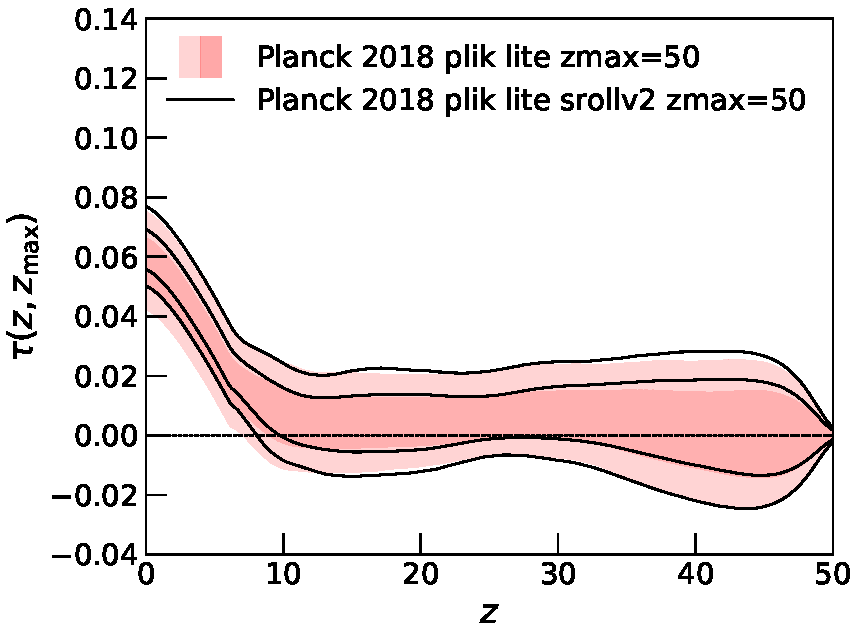
\includegraphics[width=0.65\textwidth]{results/direct_mcmc/pl18_plots_zmax50/plot_pub_tau_gtz_dz_0p1_pl18_pc_zmax50_pliklite_post_and_pl18_pc_zmax50_pliklite_srollv2.pdf}
\caption{PC chains for zmax = 50. Planck 2018 original lowE vs srollv2 likelihood (plik\_lite\_TTTEEE + lowl + simall\_EE vs plik\_lite\_TTTEEE + lowl + sroll2\_EE).
}
\label{fig:}
\end{figure}


\begin{figure}
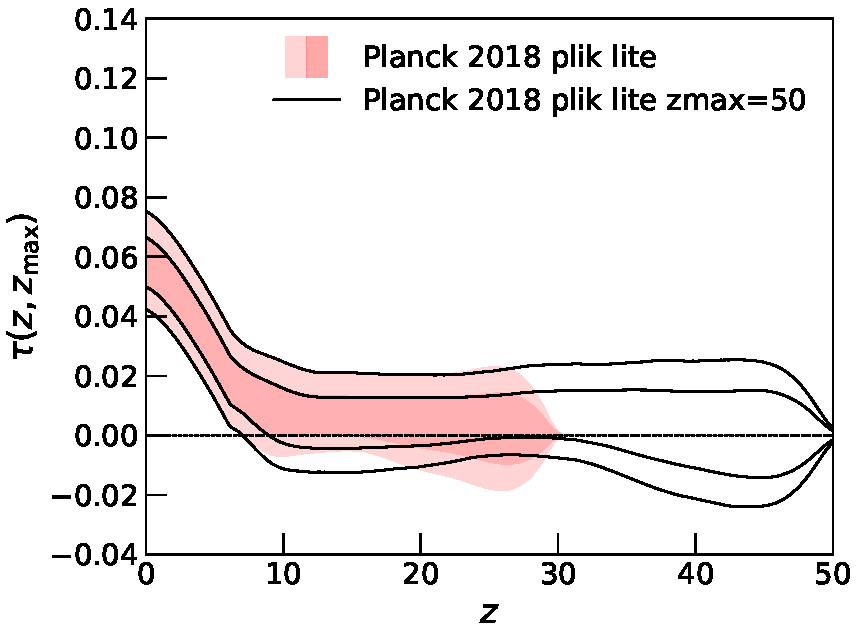
\includegraphics[width=0.65\textwidth]{results/direct_mcmc/pl18_plots_zmax30/plot_pub_tau_gtz_dz_0p1_pl18_pc_zmax30_pliklite_post_0930_and_pl18_pc_zmax50_pliklite_post.pdf}
\caption{Comparing zmax = 30 and 50 PC chains using Planck 2018 original lowE likelihood (plik\_lite\_TTTEEE + lowl + simall\_EE). Note that the zmax = 30 uses 5 PCs, whereas the zmax = 50 chains uses 7 PCs.
}
\label{fig:tau_gtz_zmax_30_vs_50_simall_EE}
\end{figure}


\begin{figure}
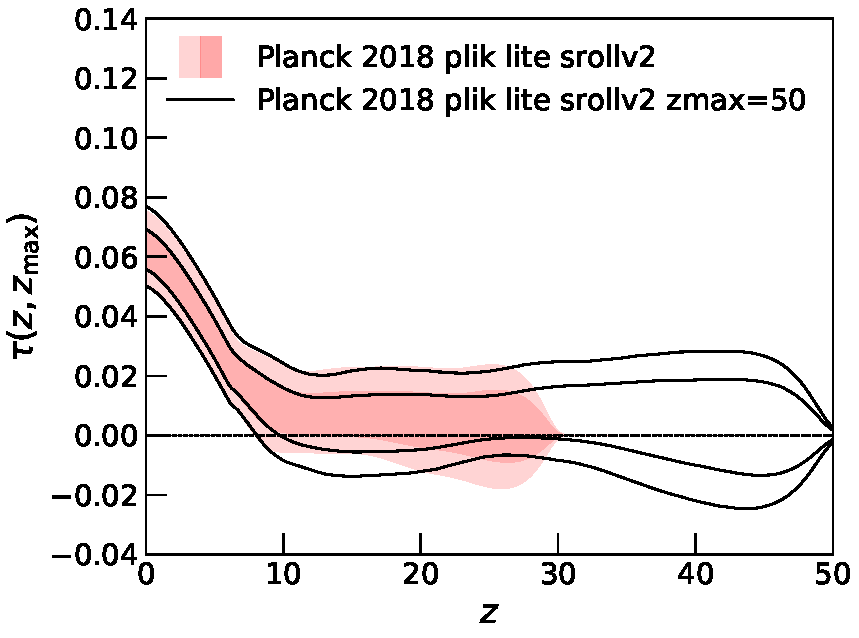
\includegraphics[width=0.65\textwidth]{results/direct_mcmc/pl18_plots_zmax30/plot_pub_tau_gtz_dz_0p1_pl18_pc_zmax30_pliklite_srollv2_0930_and_pl18_pc_zmax50_pliklite_srollv2.pdf}
\caption{Same as Fig.~\ref{fig:tau_gtz_zmax_30_vs_50_simall_EE}, but for the srollv2 likelihood (plik\_lite\_TTTEEE + lowl + sroll2\_EE).
}
\label{fig:}
\end{figure}

%Optional
\begin{figure}
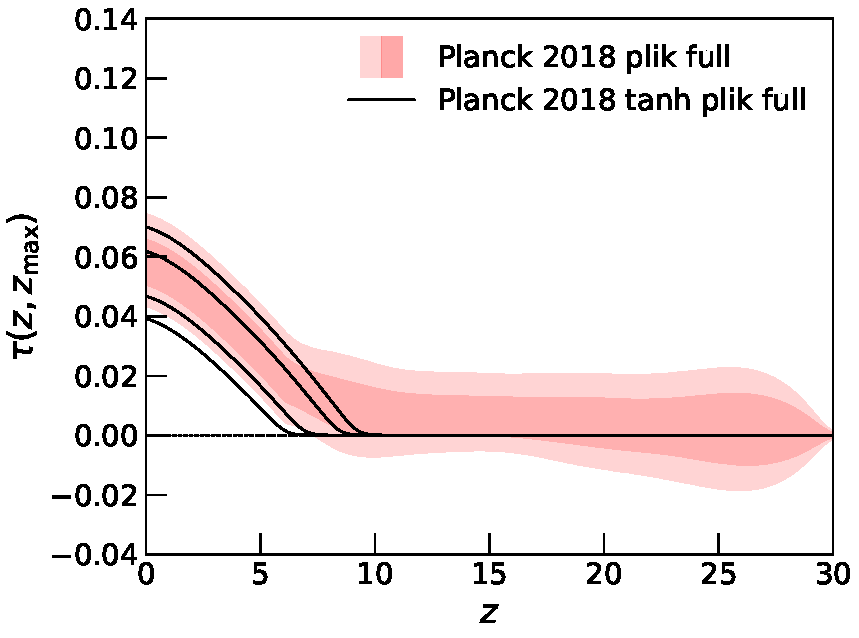
\includegraphics[width=0.65\textwidth]{results/direct_mcmc/pl18_plots_zmax30/plot_pub_tau_gtz_dz_0p1_pl18_pc_zmax30_plikfull_and_pl18_tanh_post_plikfull.pdf}
\caption{PC zmax = 30 vs tanh chains with plik\_full\_TTTEEE for the high-l likelihood.
}
\label{fig:}
\end{figure}


\begin{figure}
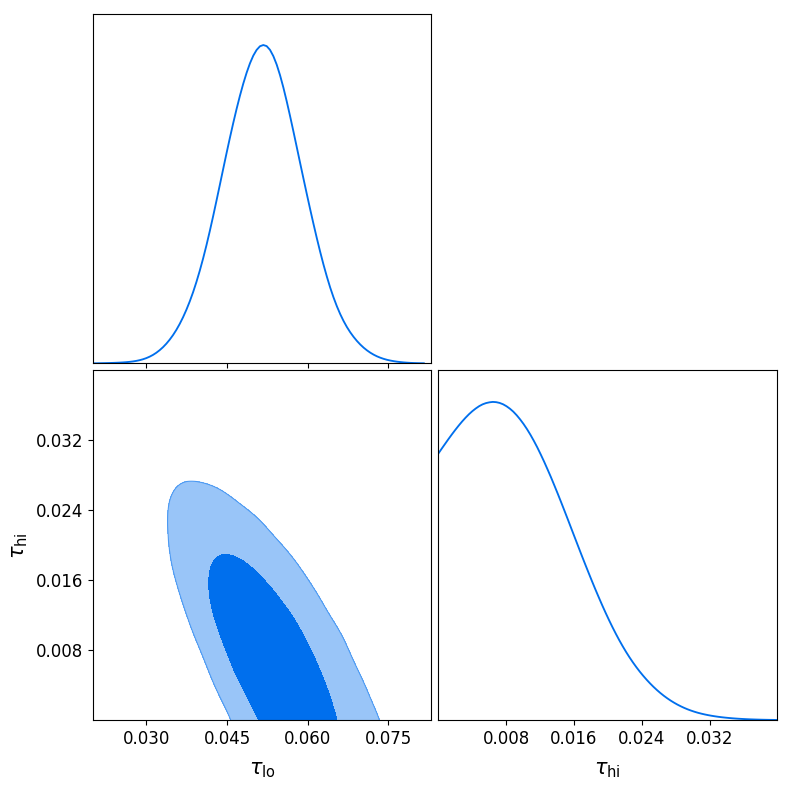
\includegraphics[width=0.65\textwidth]{results/direct_mcmc/two_parameter_model/tauhi_taulo_chains/pl18_tanh_highz_test2_run1_tri.png}
\caption{Direct MCMC chains of the two-parameter model with \tauhi and \taulo: triangle plot of \tauhi and \taulo. The marginalized 1D constraints are \taulo = $0.0516 \pm 0.0076$, \tauhi = $0.0100 \pm   0.0066$. The ML model is \taulo = 0.0543 and \tauhi = 0.0054 corresponding to $z_{\rm re} = 7.68$ and $x_{e, \mathrm{min}} = 0.021$.
}
\label{fig:two_parameter_model_2D_plot}
\end{figure}

 \begin{figure}
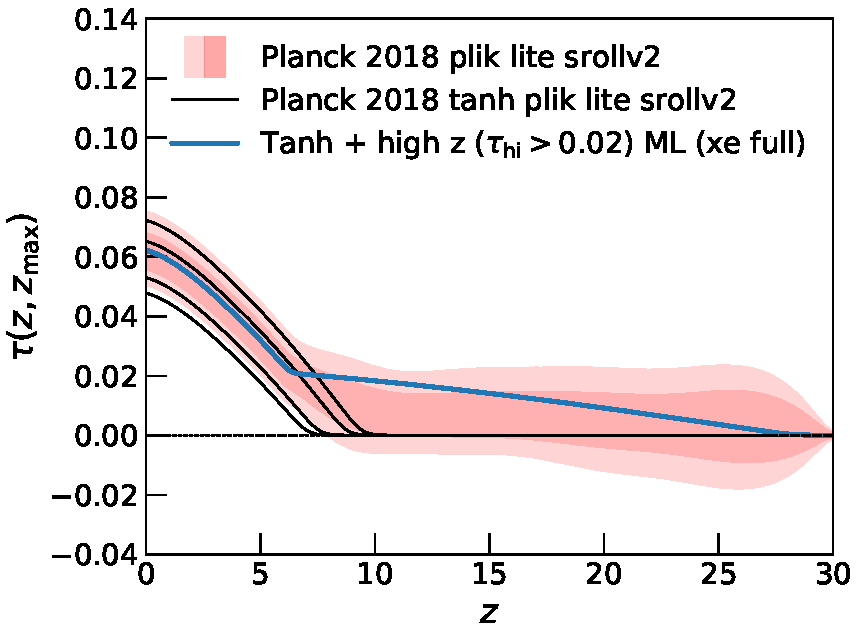
\includegraphics[width=0.65\textwidth]{   results/direct_mcmc/pl18_plots_zmax30/plot_pub_tau_gtz_dz_0p1_pl18_pc_zmax30_pliklite_srollv2_0930_and_pl18_tanh_post_pliklite_srollv2_with_added_two_parameter_ML_xe_full.pdf}
\caption{PC zmax = 30 vs tanh chains with plik lite and srollv2, with ML model from two-parameter model for \tauhi restricted to $>$ 0.02 (ML model: \tauhi = 0.0206, \taulo = 0.0414). (Note: I need to update the xe(z) curve to be that of the best-fit model in the best-fit search with tau_hi = 0.02 fixed.)
}
\label{fig:two_parameter_model_ML}
\end{figure}

\begin{figure}
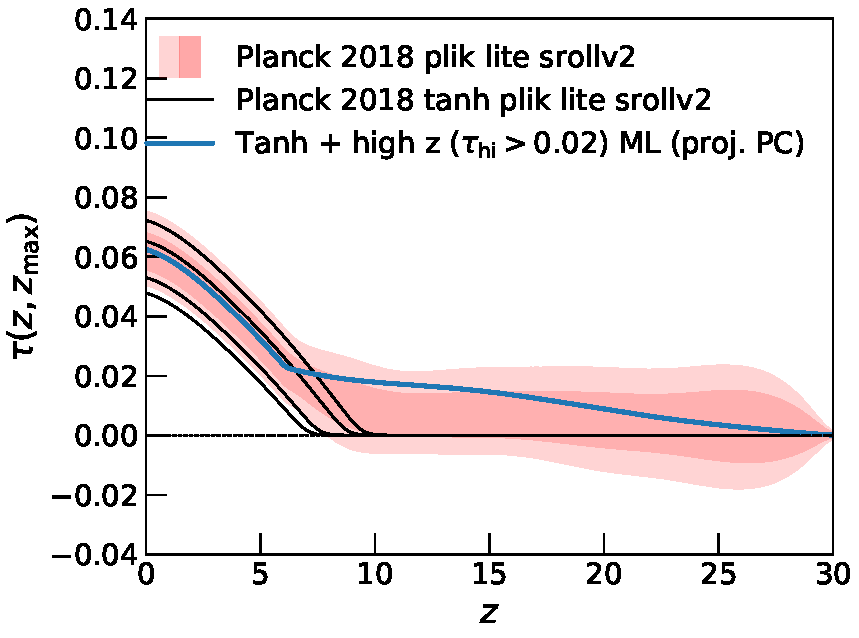
\includegraphics[width=0.65\textwidth]{  results/direct_mcmc/pl18_plots_zmax30/plot_pub_tau_gtz_dz_0p1_pl18_pc_zmax30_pliklite_srollv2_0930_and_pl18_tanh_post_pliklite_srollv2_with_added_two_parameter_ML_PC_proj.pdf}
\caption{Same as Fig.~\ref{fig:two_parameter_model_ML} except the blue curve is a PC projection instead of the full xe(z) of the model.
}
\label{fig:}
\end{figure}

\begin{figure}
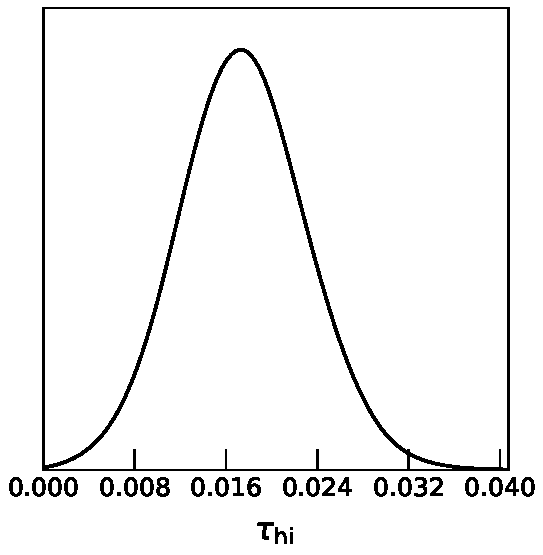
\includegraphics[width=0.65\textwidth]{   results/direct_mcmc/two_parameter_model/fixed_taulo_chains/plot_1D_tau_hi_pl18_tanh_highz_fixed_taulo_test2_run1.pdf}
\caption{Chains for two-parameter model with fixed \taulo = 0.04: 1D distribution of \tauhi (not sure what this is for anymore...).}
\label{fig:}
\end{figure}


\begin{figure}
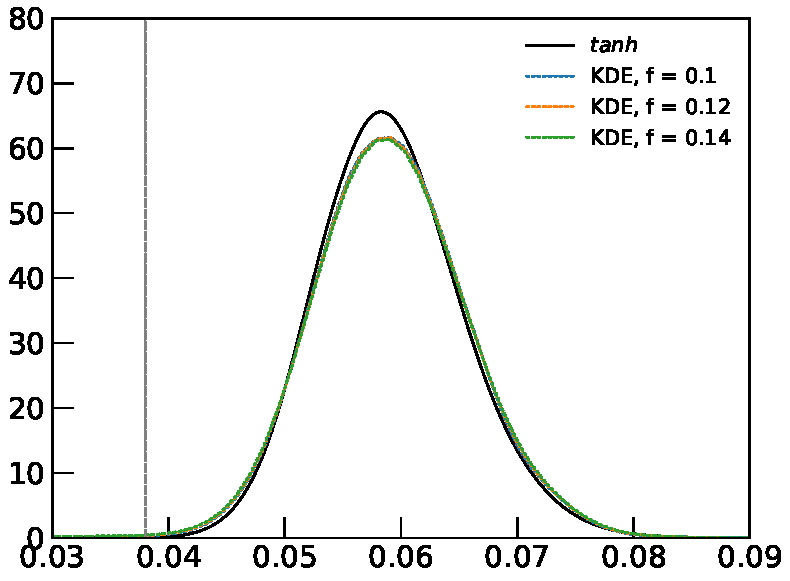
\includegraphics[width=0.65\textwidth]{python_kde/pl18_pc_zmax30_pliklite_srollv2_1015_tau_posterior_fraccov_1p0_burnin_10000_yes_norm_gaussian0p1_0p12_0p14.pdf}
\caption{KDE tests in python for the tanh model with various f = 0.1, 0.12, 0.14. It is probably safest to use any of these, so given the smaller f the better, f = 0.1 is probably the best choice here.
}
\label{fig:}
\end{figure}





\bibliography{rei.bib}

\end{document}
